% ============================================================
%  Progress Report — Transport-Metric Skill Discovery (TMSD)
%  Self-contained Beamer deck: all figures are TikZ/pgfplots,
%  no external image files needed. Paste into Overleaf and compile
%  (pdfLaTeX, TeX Live 2022+).
% ============================================================
\documentclass[aspectratio=169,11pt]{beamer}

\usetheme{metropolis}          % falls back gracefully; or use \usetheme{default}
\usepackage{pgfplots}
\pgfplotsset{compat=1.17}
\usepackage{tikz}
\usetikzlibrary{arrows.meta,positioning,shapes.geometric,calc,fit,backgrounds}
\usepackage{booktabs}
\usepackage{amsmath,amssymb,bm}
\usepackage{xcolor}
\usepackage{graphicx}
\graphicspath{{figures/}}

\definecolor{okgreen}{RGB}{46,139,87}
\definecolor{badred}{RGB}{205,72,54}
\definecolor{oursblue}{RGB}{56,101,190}
\definecolor{softgray}{RGB}{120,120,130}
\definecolor{golden}{RGB}{196,148,32}

\newcommand{\ok}[1]{\textcolor{okgreen}{#1}}
\newcommand{\bad}[1]{\textcolor{badred}{#1}}
\newcommand{\ours}[1]{\textcolor{oursblue}{#1}}

\title{Skills Nobody Taught:\\ Unsupervised Skill Discovery for Manipulating Granular Media}
\subtitle{Progress report — Transport-Metric Skill Discovery (TMSD)}
\author{Azfar Azdi Arfakhsyad}
\date{July 2026}

\begin{document}
\maketitle

% ------------------------------------------------------------
\begin{frame}{The story in one slide}
\begin{enumerate}
  \item \textbf{The dream:} robots that \emph{invent} their own useful behaviors --- no rewards, no demonstrations.
  \item \textbf{The field:} three generations of methods (DIAYN $\to$ DADS $\to$ METRA), each fixing the last one's flaw.
  \item \textbf{The gap:} none of them can manipulate \emph{stuff} --- soil, dough, sand. They learn to move \emph{themselves}.
  \item \textbf{Our idea:} measure skill diversity by the \emph{physical cost of moving material} (optimal transport / Wasserstein), computed \emph{only} on the material.
  \item \textbf{What we found:} half our hypothesis died honestly, the other half is the strongest result --- and the post-mortem produced a unifying theory of \emph{why} each method family fails on materials.
  \item \textbf{The demo:} an excavator that taught itself to dig, and executes ``dig here, dump there'' orders it was never trained on.
\end{enumerate}
\end{frame}

\begin{frame}{Roadmap}
\tableofcontents
\end{frame}

% ============================================================
\section{Background: teaching robots without teaching}
% ============================================================

\begin{frame}{What is unsupervised skill discovery?}
\textbf{Ordinary RL:} an engineer writes a reward function ($+1$ for a full bucket, $-0.01$ per second\ldots), the robot maximizes it. Every new task $\Rightarrow$ new reward $\Rightarrow$ new training.

\bigskip
\textbf{Unsupervised skill discovery (USD):} give the robot \emph{no reward at all}. Instead give it a ``skill knob'' $z$ (a vector it is handed at the start of each attempt) and one meta-instruction:

\begin{center}
\emph{``Behave so differently for different $z$ that an observer could tell which $z$ you were given.''}
\end{center}

\bigskip
Like a child alone in a sandbox: nobody defines ``dig'' or ``pile'' --- distinct, repeatable behaviors emerge from the drive to do \emph{distinguishable things}. Afterwards, the skill knob becomes a \emph{control interface}: point $z$ at what you want.
\end{frame}

\begin{frame}{The formal skeleton (shared by every method)}
\begin{itemize}
  \item Skill $z \sim p(z)$ fixed for an episode; policy $\pi(a \mid s, z)$.
  \item Learn $\pi$ to maximize an \textbf{intrinsic} (self-generated) reward measuring how \emph{informative about $z$} the visited states are.
  \item The methods differ in exactly one thing: \textbf{what ``different'' means}.
\end{itemize}
\begin{center}
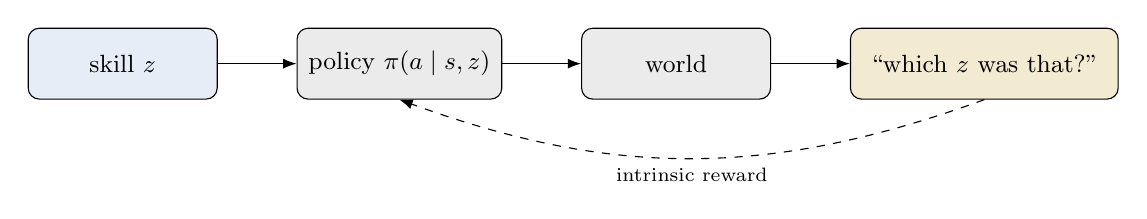
\begin{tikzpicture}[node distance=6mm and 10mm, every node/.style={font=\small}]
  \node[draw, rounded corners, fill=oursblue!12, minimum width=2.4cm, minimum height=0.9cm] (z) {skill $z$};
  \node[draw, rounded corners, fill=softgray!15, minimum width=2.6cm, minimum height=0.9cm, right=of z] (pi) {policy $\pi(a\mid s,z)$};
  \node[draw, rounded corners, fill=softgray!15, minimum width=2.4cm, minimum height=0.9cm, right=of pi] (env) {world};
  \node[draw, rounded corners, fill=golden!20, minimum width=3.4cm, minimum height=0.9cm, right=of env] (disc) {``which $z$ was that?''};
  \draw[-Latex] (z) -- (pi);
  \draw[-Latex] (pi) -- (env);
  \draw[-Latex] (env) -- (disc);
  \draw[-Latex, dashed] (disc.south) to[bend left=20] node[below, font=\scriptsize]{intrinsic reward} (pi.south);
\end{tikzpicture}
\end{center}
\end{frame}

% ============================================================
\section{Three generations of methods, three definitions of ``different''}
% ============================================================

\begin{frame}{Generation 1 --- DIAYN (2019): ``be identifiable''}
\textbf{Idea.} Maximize the mutual information $I(S;Z)$: train a discriminator $q(z \mid s)$ that guesses the skill from the state; reward the policy when the guess is easy.
\[
r \;=\; \log q(z \mid s) \;-\; \log p(z)
\]
\textbf{What emerges.} Distinct poses and gaits --- genuinely different behaviors, zero supervision. Landmark result.

\bigskip
\textbf{The flaw.} \emph{Identifiable} $\neq$ \emph{substantial}. A skill is perfectly identifiable if it tilts one joint by $1^\circ$ and holds still. MI is maximized by \textbf{microscopic, static differences} --- there is no pressure to \emph{keep changing} the world. (We will meet this flaw again, measured, on soil.)
\end{frame}

\begin{frame}{Generation 2 --- DADS (2020): ``be predictable''}
\textbf{Idea.} Skills should have consequences you can \emph{model}. Learn skill-conditioned dynamics $q(s' \mid s, z)$ and reward transitions that are predictable under your own $z$ but unlike other skills' transitions:
\[
r \;=\; \log q(s' \mid s, z) \;-\; \log \tfrac{1}{L}\textstyle\sum_{l} q(s' \mid s, z_l)
\]
\textbf{What emerges.} Smooth, model-friendly locomotion primitives; enables planning in skill space.

\bigskip
\textbf{The flaw.} The signal lives in \textbf{per-step state changes}. If the interesting part of the world changes rarely or slowly, every skill's next state is equally (perfectly) predictable --- the two terms cancel and the reward \textbf{evaporates}. (We measured exactly this on soil: reward $\equiv 0.000$ for 200{,}000 steps.)
\end{frame}

\begin{frame}{Generation 3 --- METRA (2024): ``go far''}
\textbf{Idea.} Stop asking ``identifiable?'' and ask ``\emph{far apart}?''. Learn a map $\phi$ of states into a latent space and make skills travel in different latent directions:
\[
\max_{\pi,\phi}\; \mathbb{E}\big[(\phi(s') - \phi(s))^{\!\top} z\big]
\quad \text{s.t.} \quad \|\phi(s) - \phi(s')\| \le d(s, s'),
\]
where $d$ is a distance between states (METRA uses \emph{temporal} distance: how many steps to get from one state to the other). The constraint stops $\phi$ from cheating by inflating distances.

\medskip
\textbf{Key property.} The per-step rewards \emph{telescope}:
\[
\textstyle\sum_t (\phi(s_{t+1})-\phi(s_t))^{\top} z \;=\; (\phi(s_T) - \phi(s_0))^{\top} z .
\]
Total reward $=$ \textbf{net displacement}. You cannot earn it by micro-wiggling; you must \emph{cumulatively change the world}. State of the art on locomotion.

\medskip
\textbf{The remaining flaw$\ldots$}
\end{frame}

\begin{frame}{The gap all three share: they move \emph{themselves}, not \emph{stuff}}
The state $s$ contains everything --- joint angles, velocities, \emph{and} the world outside. The richest, easiest-to-vary part of $s$ is the robot's \textbf{own body}. All three objectives happily feast on it.

\begin{quote}
``Previous approaches only learn to gain control of the agent's own body, \emph{completely ignoring the object}.'' --- the CSD authors (ICML 2023), on DIAYN/LSD in a manipulation task
\end{quote}

\textbf{And nobody has tried materials.} Skill discovery is confined to rigid bodies and locomotion. Meanwhile the hard, valuable frontier of robotics is \emph{deformable and granular matter}: soil, dough, sand, grain --- where writing rewards by hand is hardest, i.e.\ exactly where USD would matter most.

\bigskip
\begin{center}
\textbf{Open question we attacked:} \emph{can a robot invent manipulation of a material --- digging, piling, shaping --- with zero supervision?}
\end{center}
\end{frame}

% ============================================================
\section{Our idea: measure diversity in units of moved material}
% ============================================================

\begin{frame}{Wasserstein distance, intuitively: the earth mover}
Suppose the world state is a \emph{pile of sand}, described by how much mass sits at each location. How different are two piles?

\begin{center}
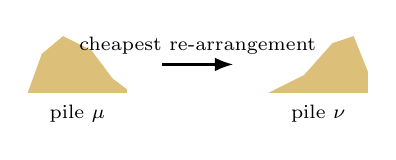
\begin{tikzpicture}[scale=0.9, every node/.style={font=\scriptsize}]
  % pile A
  \fill[golden!60] (0,0) -- (0.2,0.55) -- (0.5,0.8) -- (0.9,0.6) -- (1.2,0.2) -- (1.4,0.05) -- (1.4,0) -- cycle;
  \node at (0.7,-0.3) {pile $\mu$};
  % arrow
  \draw[-Latex, thick] (1.9,0.4) -- (2.9,0.4) node[midway, above]{cheapest re-arrangement};
  % pile B
  \fill[golden!60] (3.4,0) -- (3.6,0.1) -- (3.9,0.25) -- (4.3,0.7) -- (4.6,0.8) -- (4.8,0.3) -- (4.8,0) -- cycle;
  \node at (4.1,-0.3) {pile $\nu$};
\end{tikzpicture}
\end{center}

The \textbf{Wasserstein distance} $W_2(\mu,\nu)$ is the minimum total \emph{work} --- mass $\times$ distance --- a perfect bulldozer would need to convert one pile into the other. It is also called the \emph{earth mover's distance}, and for once the metaphor is literal: \textbf{our robot is the earth mover.}

\medskip
Contrast: a pixel-by-pixel (Euclidean) comparison calls two piles ``very different'' even when one is just the other shifted 10\,cm --- it has no idea that moving mass \emph{far} costs more than moving it \emph{near}.
\end{frame}

\begin{frame}{Wasserstein distance, mathematically}
For probability measures $\mu,\nu$ on $\mathbb{R}^n$ (Kantorovich formulation):
\[
W_2(\mu,\nu) \;=\; \Big( \min_{\gamma \,\in\, \Pi(\mu,\nu)} \int \|x-y\|^2 \, d\gamma(x,y) \Big)^{1/2},
\]
where $\Pi(\mu,\nu)$ is the set of \emph{transport plans} (joint distributions with marginals $\mu$, $\nu$): $\gamma(x,y)$ says how much mass travels from $x$ to $y$.

\medskip
\textbf{The 1D gift.} On a line, the optimal plan never lets mass streams cross, so it is given by matching quantiles. With CDFs $F_\mu, F_\nu$ and quantile functions $F^{-1}$:
\[
W_2^2(\mu,\nu) \;=\; \int_0^1 \big( F_\mu^{-1}(u) - F_\nu^{-1}(u) \big)^2 \, du .
\]
\emph{Closed form. No optimization. Microseconds on a GPU.} Our soil bed is (to first order) a 1D mass profile over $x$ --- so we get the exact physical metric essentially for free, thousands of times per second during training.
\end{frame}

\begin{frame}{Transport-Metric Skill Discovery (TMSD): the two ingredients}
Take METRA's template and change \emph{two things}:

\begin{enumerate}
  \item \textbf{Physical ground metric.} Set $d(s,s') = W_2(\mu_s, \mu_{s'})$ --- the transport cost between the \emph{soil mass distributions}. Latent displacement is then bounded by \emph{tons-moved-times-meters}:
  \[
  \max_{\pi,\phi}\; \mathbb{E}\big[(\phi(\mu') - \phi(\mu))^{\top} z\big]
  \quad \text{s.t.} \quad \|\phi(\mu)-\phi(\mu')\| \le W_2(\mu, \mu').
  \]
  \item \textbf{External-state conditioning.} $\phi$ sees \emph{only the soil} --- never a joint angle, never a velocity. A skill that merely waves the arm produces $\phi(\mu')=\phi(\mu)$: \textbf{reward exactly zero, by construction}.
\end{enumerate}

\medskip
Hypothesis going in: ingredient 1 (the metric) is the headline, ingredient 2 is plumbing.\\
\textbf{Reality (spoiler): precisely backwards --- and proving that took 33 training runs.}
\end{frame}

\begin{frame}{Testbed: a 2D excavator on granular physics}
\begin{columns}
\column{0.55\textwidth}
\begin{itemize}
  \item Custom DEM simulation: $\sim$1200 soil grains, Hertz contacts, friction, cohesion; CUDA backend.
  \item 3-joint hydraulic arm (boom/stick/bucket) with realistic torque limits; fixed base.
  \item Observation: proprioception $+$ soil heightfield. Action: 3 joint velocities.
  \item Soil measure $\mu$: mass histogram over $x$ (64 bins), \textbf{conserved} $\Rightarrow$ balanced optimal transport is well-posed.
  \item Skills: continuous $z$ on the unit sphere, $\dim = 4$.
\end{itemize}
\column{0.42\textwidth}
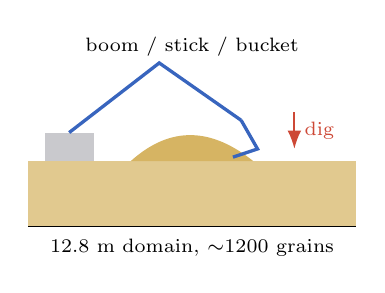
\begin{tikzpicture}[scale=0.52, every node/.style={font=\scriptsize}]
  % ground
  \fill[golden!50] (0,0) rectangle (8,1.6);
  \fill[golden!70] (2.5,1.6) .. controls (3.5,2.5) and (4.5,2.4) .. (5.5,1.6);
  % machine
  \fill[softgray!40] (0.4,1.6) rectangle (1.6,2.3);
  \draw[very thick, oursblue] (1.0,2.3) -- (3.2,4.0) -- (5.2,2.6);
  \draw[very thick, oursblue] (5.2,2.6) -- (5.6,1.9) -- (5.0,1.7);
  \node at (4.0,4.4) {boom / stick / bucket};
  \draw[-Latex, badred, thick] (6.5,2.8) -- (6.5,1.9) node[midway,right]{dig};
  \draw[decorate] (0,0) -- (8,0);
  \node at (4,-0.5) {12.8 m domain, $\sim$1200 grains};
\end{tikzpicture}
\end{columns}
\medskip
Everything below runs on \textbf{one desktop GPU} (RTX 5080): 33 runs, $\approx$70 GPU-hours total.
\end{frame}

\begin{frame}{Who sees what: the four-layer state representation}
\begin{center}
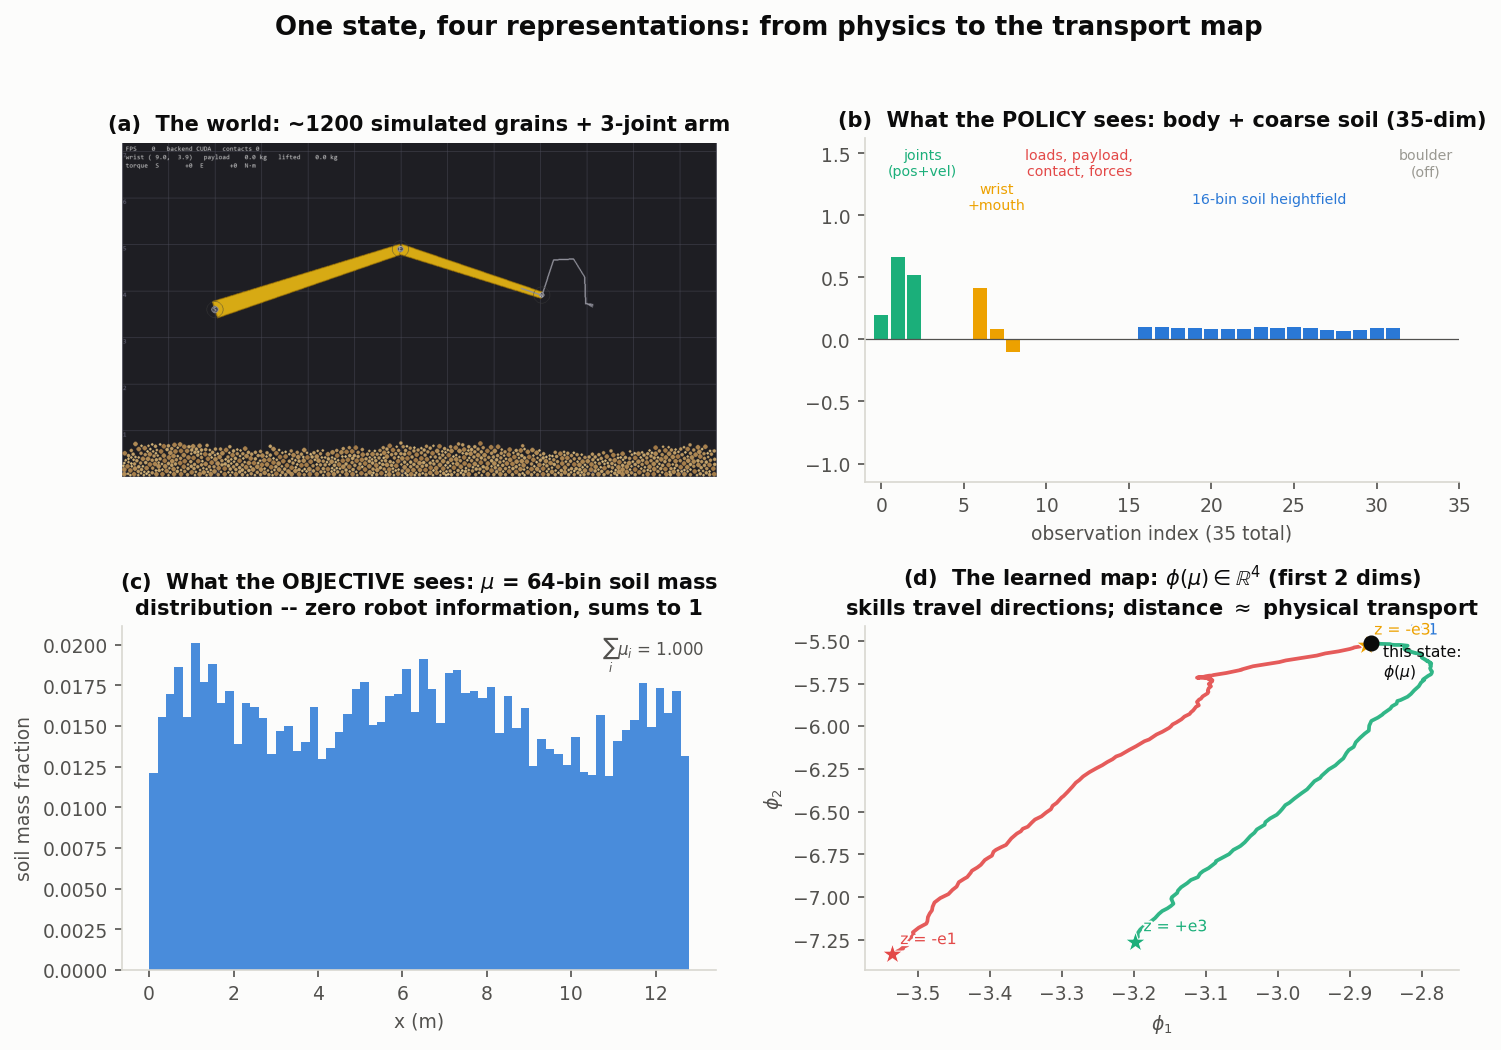
\includegraphics[height=0.72\textheight]{fig_representation.png}
\end{center}
{\scriptsize The policy (b) may know its body --- it must, to control it. The
\emph{objective's} representation $\phi$ sees only (c): the soil mass
distribution, zero robot information. (d): the learned latent map, with real
skill episodes traced. The paper's central finding lives entirely in the split
between (b) and (c).}
\end{frame}

% ============================================================
\section{The experimental campaign, step by step}
% ============================================================

\begin{frame}{Experiment 1 --- Does anything emerge at all?}
\textbf{Problem.} Nobody has shown reward-free skills on granular media. Does the objective even produce soil interaction?

\textbf{Test.} 500k steps, fixed terrain, TMSD objective ($W_2$ metric, soil-only $\phi$).

\begin{columns}
\column{0.52\textwidth}
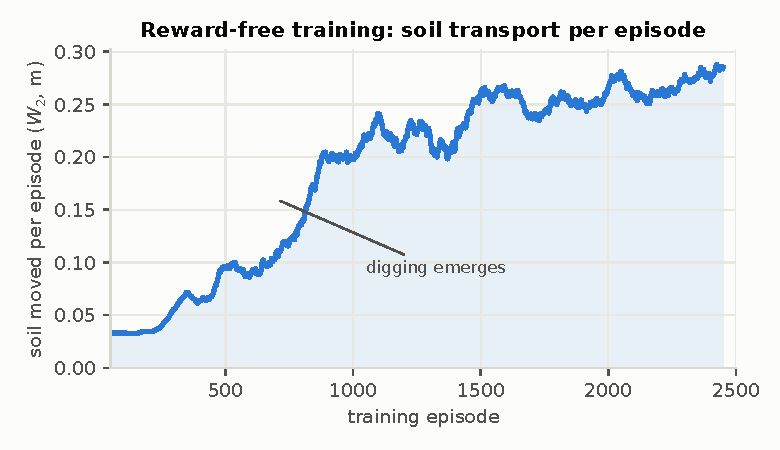
\includegraphics[width=\linewidth]{fig_learning_curve.pdf}
\column{0.46\textwidth}
\textbf{Result.} \ok{Yes.} Digging, piling, and directed mass transport emerge; late episodes move $\sim$0.27\,m of soil-mass (in $W_2$), $8\times$ the starting level, with \textbf{zero rewards}.

\medskip
\textbf{Insight.} Skill coordinate maps to physics: the sign of $z_1$ literally equals the direction the soil's center of mass shifts. The skill space \emph{is} a transport control knob.
\end{columns}
\end{frame}

\begin{frame}{Experiment 1 --- what the skills actually do to the soil}
\begin{columns}
\column{0.58\textwidth}
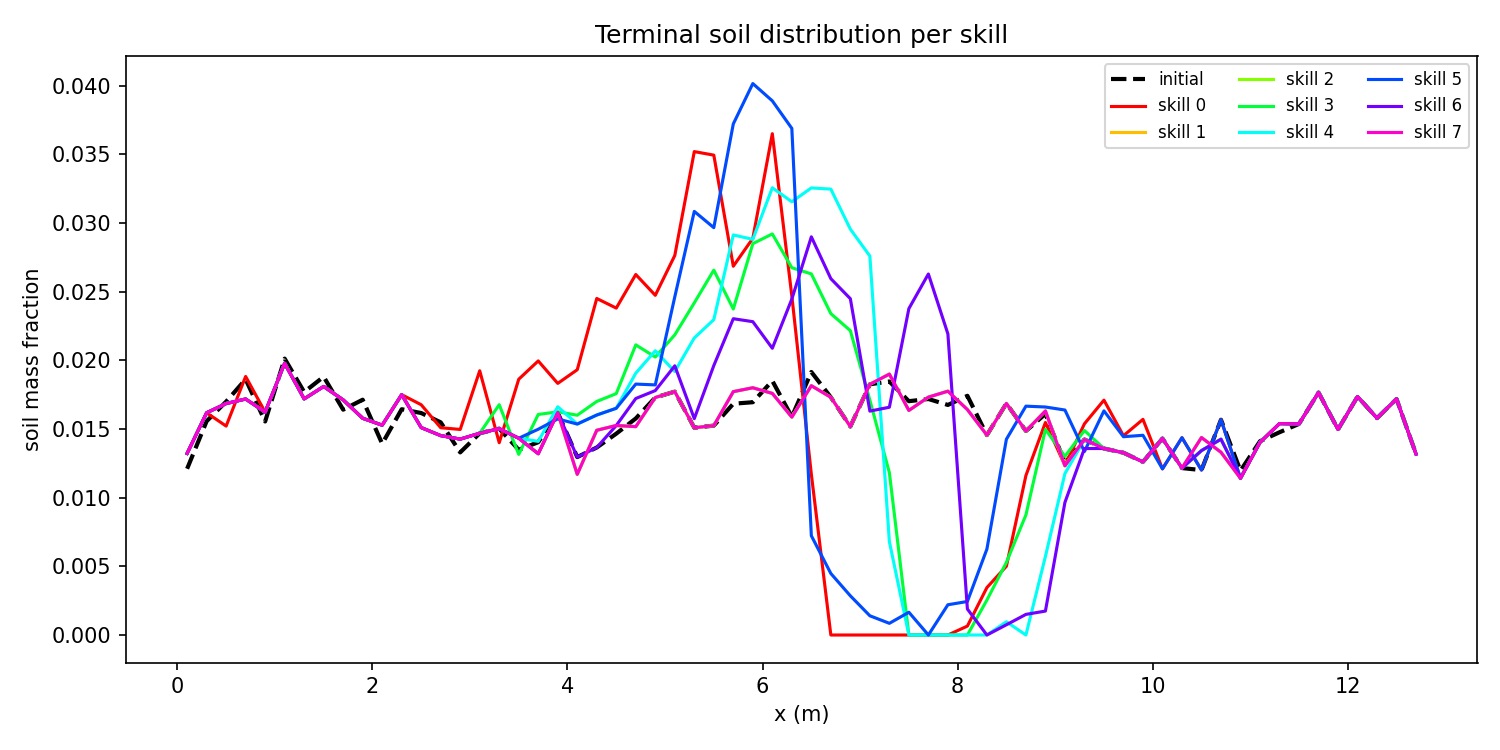
\includegraphics[width=\linewidth]{fig_terminal_profiles.png}
\column{0.40\textwidth}
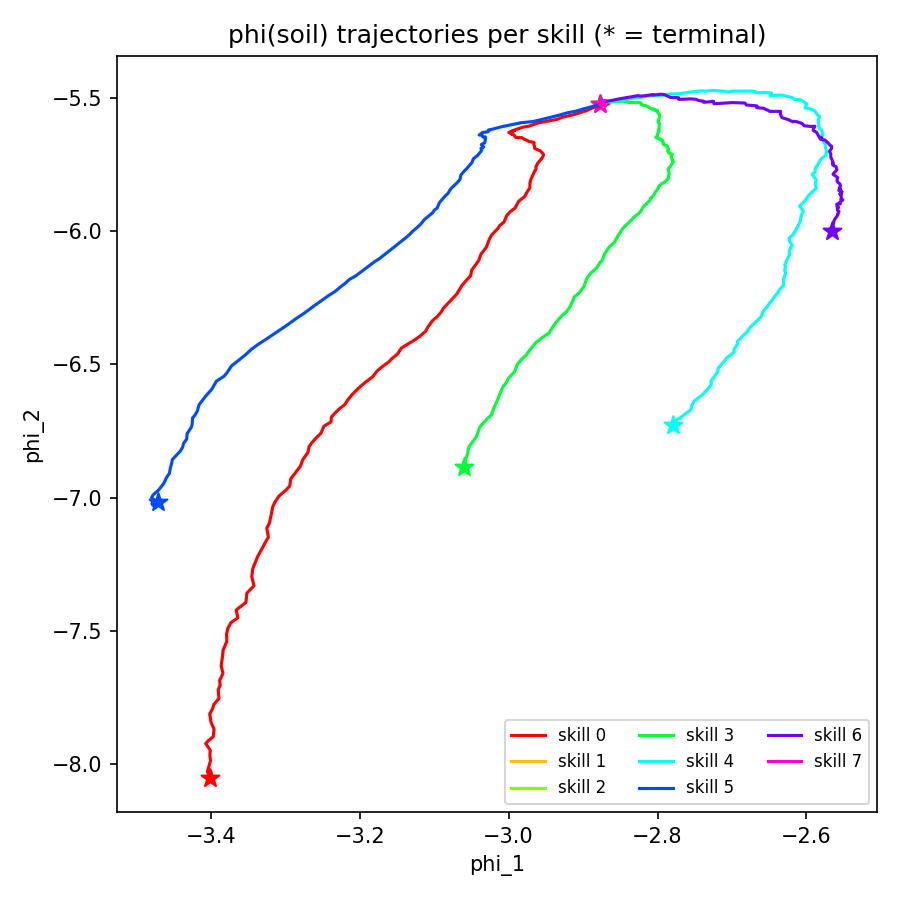
\includegraphics[width=\linewidth]{fig_phi_trajectories.png}
\end{columns}
\medskip
{\small \textbf{Left:} terminal soil profile per skill vs.\ the initial terrain (dashed) --- different skills dig and pile at different places. \textbf{Right:} the learned latent map $\phi(\text{soil})$: skill trajectories fan out in distinct directions --- the ``mental map'' of soil states, where distance $\approx$ tons moved $\times$ meters.}
\end{frame}

\begin{frame}{Experiment 2 --- Is the Wasserstein metric doing the work?}
\textbf{Problem.} Our headline claim: the \emph{physical} metric matters. A reviewer's first attack: ``this is just METRA with a different $d$.''

\textbf{Test.} Same recipe (random terrain, 3 seeds each), swap only the ground metric: $W_2$ vs.\ Euclidean-on-histograms vs.\ METRA's temporal $d\equiv1$. Judge all by the same physical yardstick.

\begin{center}
\small
\begin{tabular}{lccc}
\toprule
ground metric & $W_2$ (ours) & Euclidean & temporal (METRA) \\
\midrule
skill coverage (m, mean of 3 seeds) & $0.326 \pm 0.036$ & $0.352\pm0.034$ & $0.291\pm0.094$ \\
\bottomrule
\end{tabular}
\end{center}

\textbf{Result.} \bad{A three-way tie.} The metric hypothesis is \textbf{falsified} --- our own pre-registered ablation killed our own headline in one day.

\textbf{Insight (the good part).} Every trained $\phi$ --- regardless of metric --- ended up $0.99$-correlated with physical $W_2$. The reachable soil manifold is low-dimensional; on it, \emph{all sensible metrics agree}. Geometry is \textbf{emergent, free, and metric-agnostic}.
\end{frame}

\begin{frame}{Experiment 3 --- Then what IS doing the work?}
\textbf{Problem.} If not the metric --- is it the \emph{conditioning} (soil-only $\phi$)?

\textbf{Test.} Identical run, but let $\phi$ see the full state (proprioception $+$ soil). This \emph{is} vanilla METRA, faithfully. 3 seeds.

\begin{center}
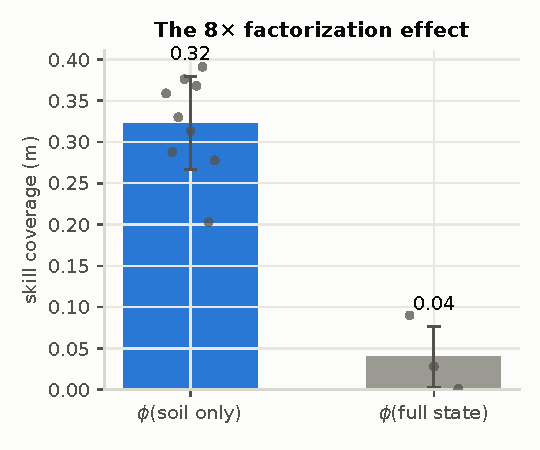
\includegraphics[height=4.6cm]{fig_factorization.pdf}
\end{center}

\textbf{Result.} \ok{$8\times$ effect.} Full-state $\phi$: 7/8 skills never touch the soil; the arm performs elaborate ``dances,'' harvesting $2000\times$ more reward \emph{per meter of soil actually moved}. The CSD failure mode, reproduced and quantified.

\textbf{Insight.} \textbf{What you show the discriminator determines what the skills are about.} The conditioning --- treated as plumbing in our ideation --- is the load-bearing ingredient.
\end{frame}

\begin{frame}{Experiment 4 --- Give the metric a fair second chance}
\textbf{Problem.} Maybe the 1D soil profile was too crude for metrics to differ. On a full 2D mass grid (deep-narrow vs.\ wide-shallow holes now distinct), transport structure should finally matter.

\textbf{Test.} 2D measure ($48\times24$ mass grid), sliced-$W_2$ (closed-form random 1D projections) vs.\ Euclidean vs.\ temporal.

\textbf{Result.} \bad{Worse than falsified.} Sliced-$W_2$: coverage $0.044$ --- \textbf{5$\times$ worse than Euclidean (0.245) on its own ruler}.

\medskip
\textbf{Insight (mechanism, from telemetry).} Not misbehavior --- \emph{starvation}: under the SW$_2$ constraint the representation extracted only $\sim$7\% of its allowed reward budget (Euclidean control: 45\%), so the policy never received a usable gradient. The physical transport metric did not mis-price soil work; it \textbf{failed to feed learning}. Honest open question, one paragraph in the paper.

\medskip
\emph{Verdict after Exp.\ 2--4: the metric claim is conclusively dead, in both regimes, with mechanisms. What survives of $W_2$: rewards in physical units (meters of mass transport) --- calibration, not performance.}
\end{frame}

\begin{frame}{Experiment 5 --- Can the skills reach \emph{goals}? (the payoff layer)}
\textbf{Problem.} Diverse skills are only useful if they compose into ``make the soil look like \emph{this}.''

\textbf{Test.} Zero-shot rule, no goal training: repeatedly command $z = \frac{\phi(\mu^{*}) - \phi(\mu_t)}{\|\cdot\|}$ toward target profile $\mu^*$. 21 targets, all trained models.

\begin{columns}
\column{0.5\textwidth}
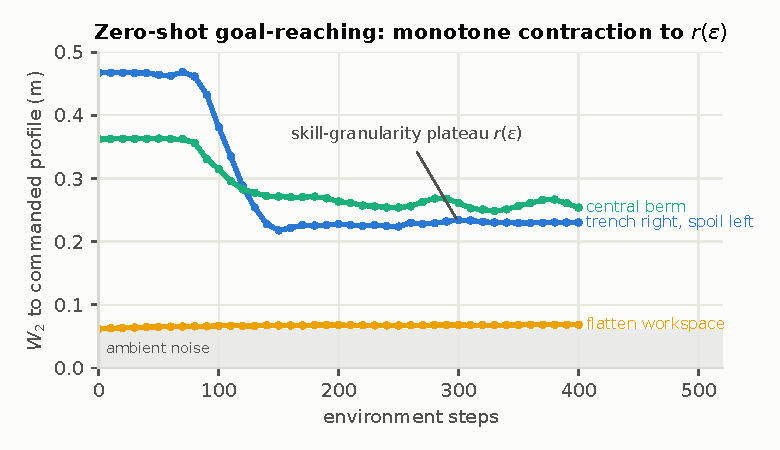
\includegraphics[width=\linewidth]{fig_contraction.pdf}
\column{0.47\textwidth}
\textbf{Result.} \ok{39--63\% of the distance-to-goal removed, zero-shot}; 79--94\% of control intervals \emph{monotonically} decrease $W_2$ --- an empirical \textbf{contraction certificate}.

\medskip
\textbf{Insight.} Curves plateau at $\approx0.23$\,m: the \emph{skill-granularity radius} $r(\varepsilon)$ our certificate theory predicts. Skills contract to a ball around the goal, not to a point --- this number will explain a later failure.
\end{columns}
\end{frame}

\begin{frame}{Experiments 6--7 --- The other families, same arena (DIAYN, DADS)}
\textbf{Problem.} Is \emph{conditioning} alone the whole story? Then DIAYN- and DADS-style objectives, given soil-only inputs, should also work.

\textbf{Test.} Full $3\times2$ grid: objective family $\times$ conditioning, 2--3 seeds per cell, identical recipe and frozen evaluation.

\begin{center}
\small
\begin{tabular}{lcc}
\toprule
\textbf{objective family} & \textbf{soil-only} & \textbf{full-state (vanilla)} \\
\midrule
distance-max (METRA-style, any metric) & \ok{$0.29$--$0.35$ \checkmark} & \bad{$0.039$ \texttimes} \\
MI discriminator (DIAYN-style) & \bad{$0.021$ \texttimes} & \bad{$0.031$ \texttimes} \\
skill dynamics (DADS-style) & \bad{$0.008$ \texttimes} & \bad{$0.130^{*}$ \texttimes} \\
\bottomrule
\end{tabular}
\end{center}

\textbf{Result.} \textbf{Only one cell works.} Neither ingredient suffices alone; both are necessary.

\textbf{Mechanisms (measured, not guessed):}
\begin{itemize}
  \item \bad{DIAYN$+$soil \emph{saturates}}: discriminator hits $0.98$ cosine accuracy off \emph{microscopic} grain differences --- identifiable without moving anything. (Gen-1 flaw, on soil.)
  \item \bad{DADS$+$soil \emph{starves}}: soil barely changes per step $\Rightarrow$ every skill's next state equally predictable $\Rightarrow$ reward $\equiv 0.000$ for the entire run. (Gen-2 flaw, on soil.)
\end{itemize}
{\scriptsize $^{*}$One full-state DADS seed reaches $0.203$ by \emph{incidental} soil contact from arm-dynamics skills (its sibling seed: $0.057$, near floor) --- still $2.5\times$ below the working family's mean, with the highest seed variance in the table.}
\end{frame}

\begin{frame}{The unifying insight: materials are \emph{slow} states}
Soil changes rarely and slowly; the arm changes richly at every step. This one property explains the whole grid:

\begin{center}
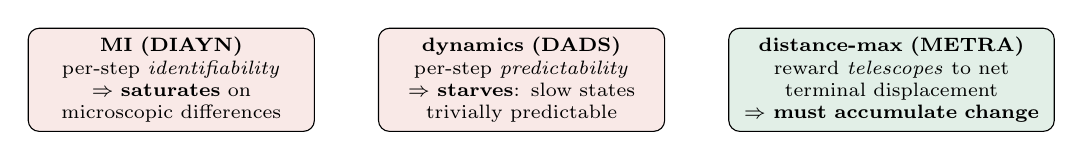
\begin{tikzpicture}[node distance=4mm and 8mm, every node/.style={font=\scriptsize}]
  \node[draw, rounded corners, fill=badred!12, text width=3.4cm, align=center] (mi)
    {\textbf{MI (DIAYN)}\\ per-step \emph{identifiability}\\ $\Rightarrow$ \textbf{saturates} on\\ microscopic differences};
  \node[draw, rounded corners, fill=badred!12, text width=3.4cm, align=center, right=of mi] (dads)
    {\textbf{dynamics (DADS)}\\ per-step \emph{predictability}\\ $\Rightarrow$ \textbf{starves}: slow states\\ trivially predictable};
  \node[draw, rounded corners, fill=okgreen!14, text width=3.9cm, align=center, right=of dads] (dm)
    {\textbf{distance-max (METRA)}\\ reward \emph{telescopes} to net\\ terminal displacement\\ $\Rightarrow$ \textbf{must accumulate change}};
\end{tikzpicture}
\end{center}

\[
\underbrace{\textstyle\sum_t (\phi(s_{t+1})-\phi(s_t))^{\top}z}_{\text{what the policy collects}}
\;=\; \underbrace{(\phi(s_T)-\phi(s_0))^{\top}z}_{\text{net change of the material}}
\]

\begin{center}
\textbf{Design law:} \emph{on slow external states, the objective must (i) integrate change over time, not score it per step, and (ii) see only that state while doing so.} Each frontier family lacks one of the two.
\end{center}
\end{frame}

\begin{frame}{Experiment 8 --- Stress test: arbitrary user goals (where it breaks)}
\textbf{Problem.} Interactive demo: user sculpts terrain freehand, records it, wrecks it, robot restores. Reality: \bad{it failed, badly.}

\textbf{Diagnosis chain} (each step measured):
\begin{enumerate}
  \item Off-distribution states? Retrained \emph{on} user-like edits $\to$ \bad{no change}.
  \item Bad skill \emph{selection}? Built a planner with \textbf{perfect lookahead} (model-predictive control using the simulator itself as the model) $\to$ \bad{$+6$--$13\%$ only}.
  \item[$\Rightarrow$] With perfect selection ruled out, the \textbf{vocabulary itself} is the limit: $\sim$3--5 coarse transport modes cannot express local repairs. And user goals sit \emph{inside} the $r(\varepsilon)\!\approx\!0.2$\,m granularity radius from Exp.\ 5 --- the method performs exactly to its certificate, and the certificate says ``too coarse for this.''
\end{enumerate}

\textbf{Insight (the honest headline):} \textbf{diversity $\neq$ controllability.} Skill discovery finds the few \emph{most mutually different} behaviors, not a dense basis of all behaviors. Its proper role --- consistent with how the literature quietly uses it --- is \emph{pretraining and coarse control}, with a task layer on top for precision. $r(\varepsilon)$ is the measurable gap between the two.
\end{frame}

% ============================================================
\section{The full comparison}
% ============================================================

\begin{frame}{Every method, one arena, one frozen ruler}
33 runs, $\approx$70 GPU-hours, identical simulation/recipe/budget (200k steps unless noted), evaluation protocol frozen \emph{before} results existed. Coverage $=$ mean pairwise $W_2$ between terminal soil states (8 fixed skills $\times$ 3 fixed terrains).

\begin{center}
\scriptsize
\begin{tabular}{llccc}
\toprule
\textbf{method} & \textbf{lineage} & \textbf{coverage (m)} & \textbf{soil/ep (m)} & \textbf{seeds} \\
\midrule
\ours{distance-max $+$ soil-only $\phi$, $W_2$ (TMSD)} & ours & $0.326\pm0.036$ & 0.21 & 3 \\
\ours{distance-max $+$ soil-only $\phi$, Euclidean} & ablation & $\bm{0.352\pm0.034}$ & 0.21 & 3 \\
\ours{distance-max $+$ soil-only $\phi$, temporal} & METRA$+$our fix & $0.291\pm0.094$ & 0.21 & 3 \\
distance-max, full-state (\textbf{= vanilla METRA}) & frontier & $0.040\pm0.046$ & 0.05 & 3 \\
MI, soil-only (DIAYN $+$ our fix) & frontier$+$fix & $0.021\pm0.015$ & 0.04 & 3 \\
MI, full-state (\textbf{$\approx$ vanilla DIAYN}) & frontier & $0.031\pm0.028$ & 0.05 & 3 \\
dynamics, soil-only (DADS $+$ our fix) & frontier$+$fix & $0.008\pm0.008$ & 0.04 & 2 \\
dynamics, full-state (\textbf{$\approx$ vanilla DADS}) & frontier & $0.130\pm0.073$ & 0.11 & 2 \\
\midrule
sliced-$W_2$ on 2D measure & ours (negative) & $0.044$ & 0.04 & 1 \\
goal-conditioned SAC from scratch & control exp. & --- (fails to learn) & --- & 1 \\
\bottomrule
\end{tabular}
\end{center}

\vspace{1mm}
{\scriptsize Networks $\sim$315k parameters each; 1.3--2.5 h per 200k-step run at 30--60 env-steps/s on one RTX 5080.}
\end{frame}

\begin{frame}{The same table as a picture}
\begin{center}
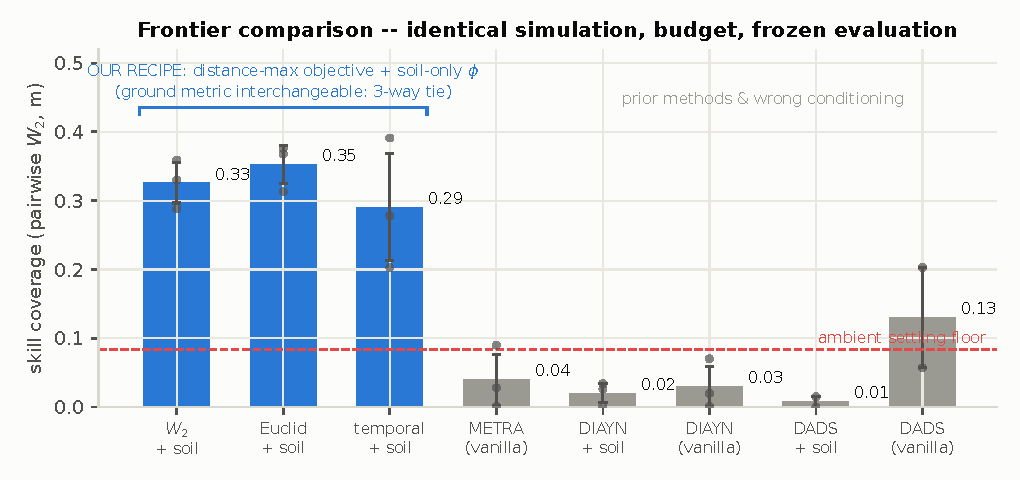
\includegraphics[width=0.88\linewidth]{fig_frontier_coverage.pdf}
\end{center}
Three blue towers, five gray stumps: the towers share both ingredients; every stump is missing at least one. Dots are individual seeds.
\end{frame}

\begin{frame}{Mechanisms, watched during training (real curves)}
\begin{center}
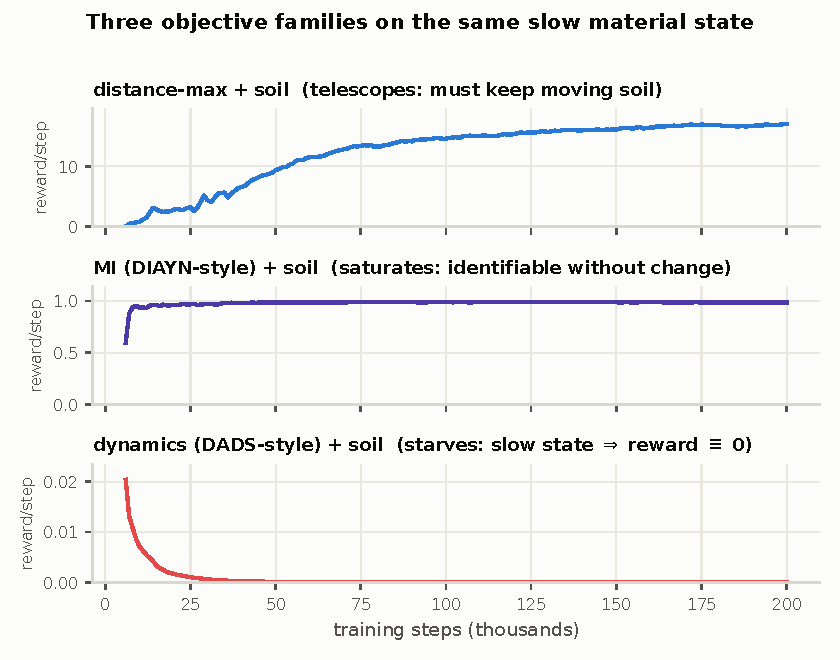
\includegraphics[height=0.78\textheight]{fig_mechanisms.pdf}
\end{center}
\end{frame}

\begin{frame}{Inside the latent spaces: the taxonomy as four axis scales}
\begin{columns}
\column{0.56\textwidth}
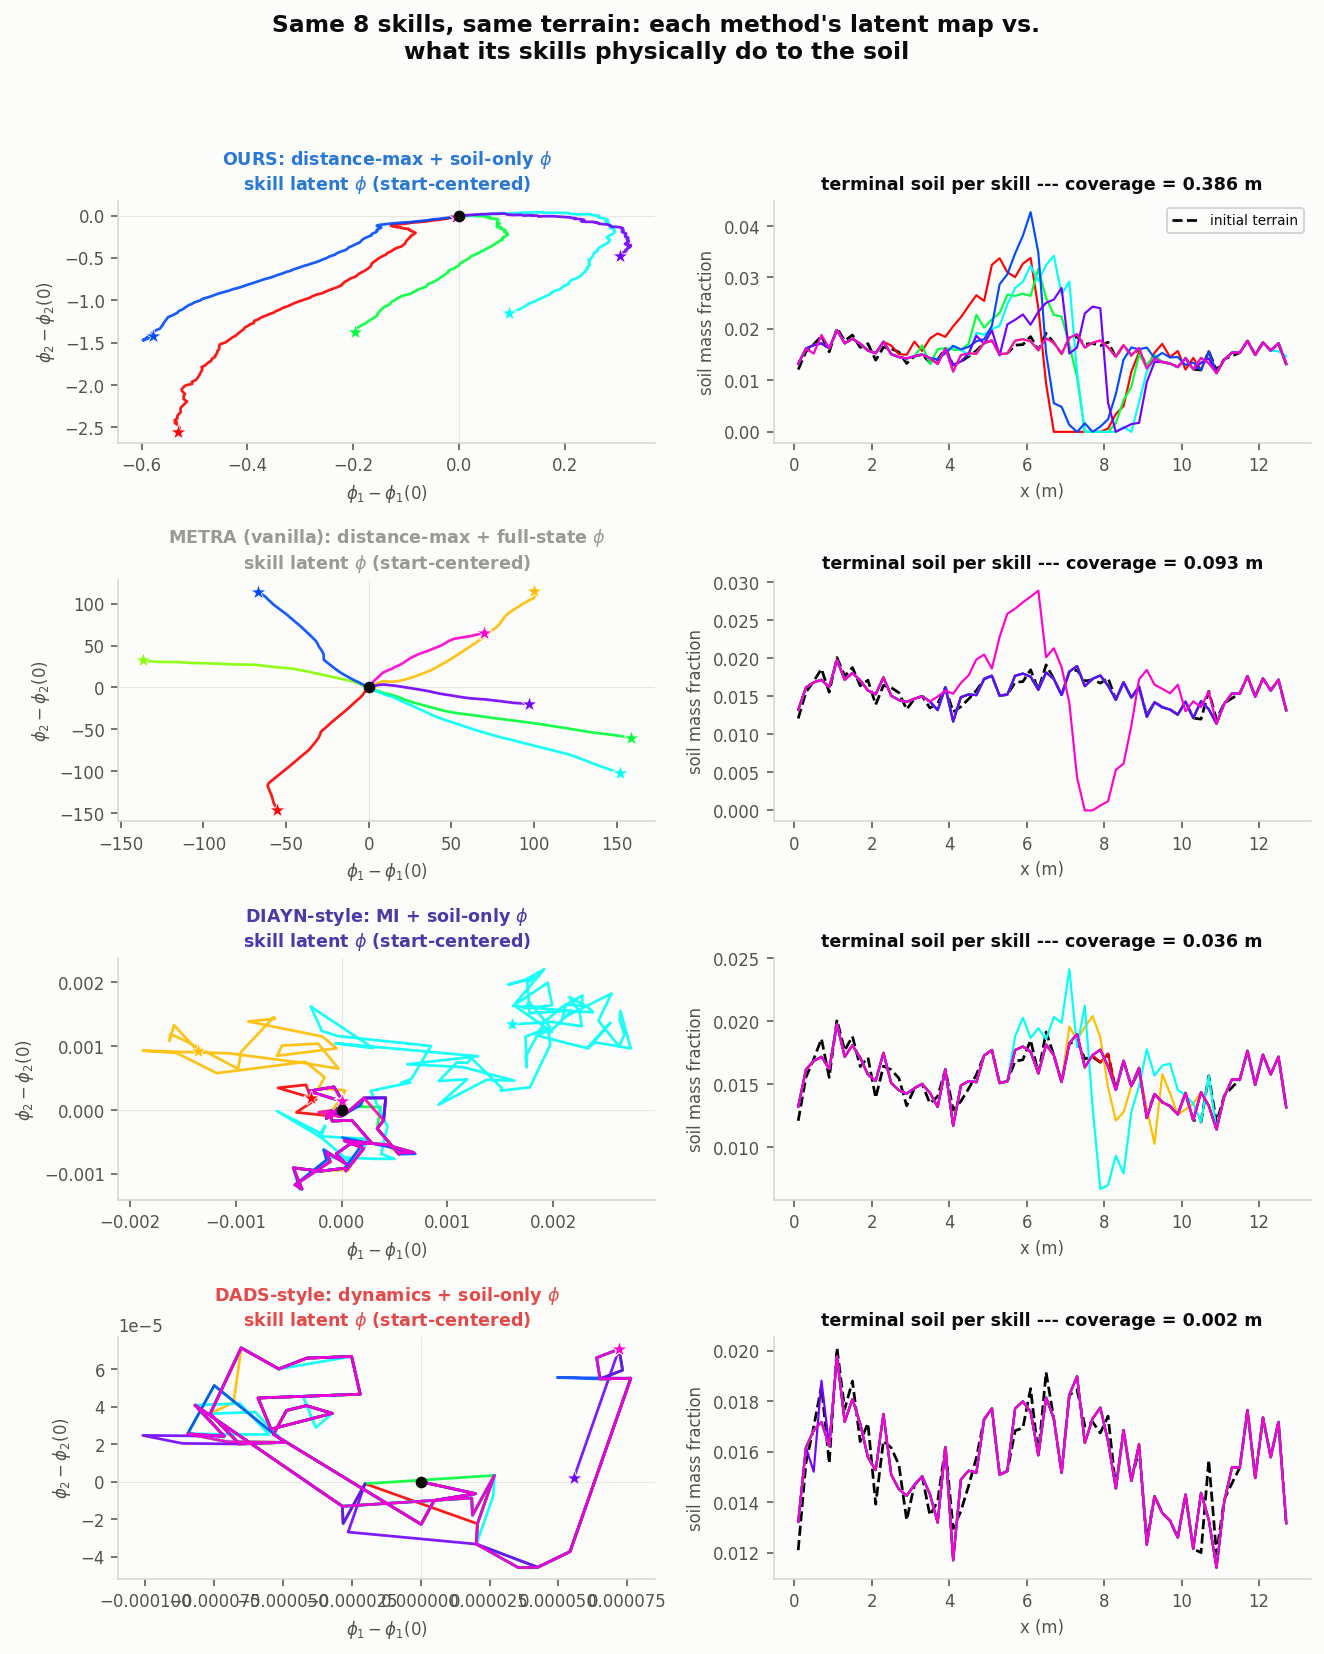
\includegraphics[width=\linewidth]{fig_latent_coverage_comparison.png}
\column{0.42\textwidth}
{\small Same 8 skills, same terrain, each method's own latent map (left) vs.\
what its skills do to the soil (right).}
\medskip

{\footnotesize
\begin{tabular}{lcc}
\toprule
 & latent spread & coverage\\
\midrule
METRA & $\sim$150 & 0.09\,m\\
\textbf{ours} & $\sim$2.5 & \textbf{0.39\,m}\\
DIAYN & $\sim$0.002 & 0.04\,m\\
DADS & $\sim$0.00007 & 0.00\,m\\
\bottomrule
\end{tabular}}
\medskip

{\small METRA: a beautiful $\pm150$ latent fan above \emph{untouched soil} ---
diversity decoupled from the world. Ours: the only row where latent geometry
and soil geometry agree, because the $W_2$ cap prices latent motion in real
mass transport.}
\end{columns}
\end{frame}

\begin{frame}{Coverage matrices: the fingerprint view (one shared color scale)}
\begin{center}
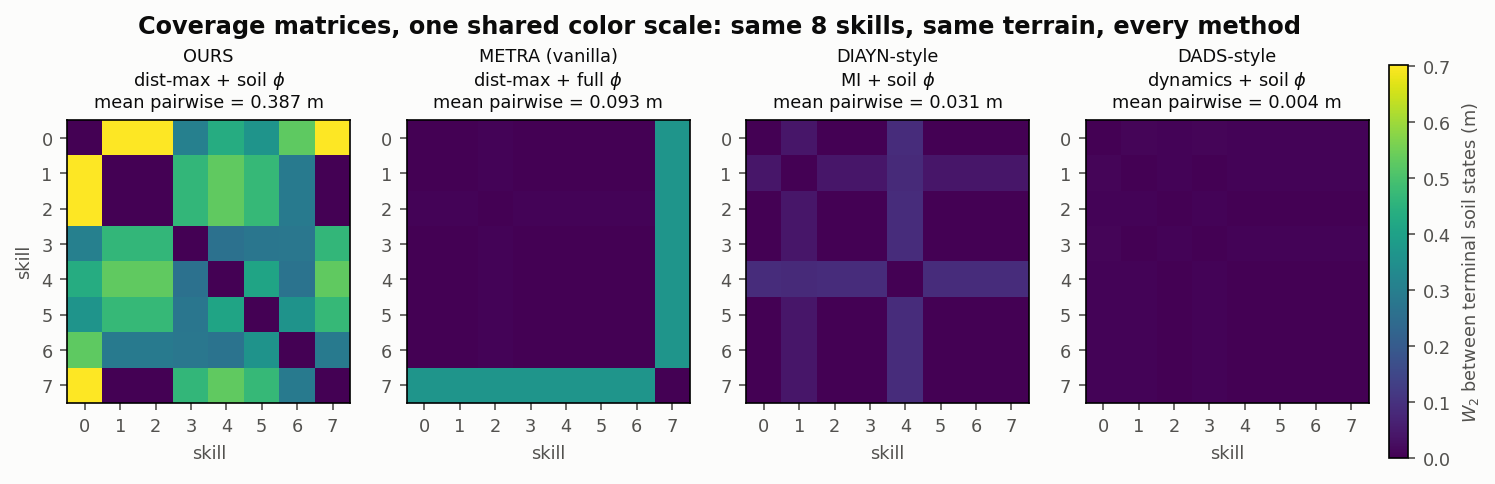
\includegraphics[width=0.98\linewidth]{fig_coverage_matrices.png}
\end{center}
{\small Bright cell $=$ that skill pair left the soil in genuinely different
states. Ours: a quilt. METRA: one bright cross --- a single working skill, seven
latent-diverse clones. DIAYN: a ghost. DADS: black. The frontier table's
coverage numbers are the means of these matrices.}
\end{frame}

\begin{frame}{What each objective is \emph{actually} paid for (mechanism fingerprints)}
Episode reward earned per meter of soil actually moved (log scale) --- a lie detector for objectives:
\begin{center}
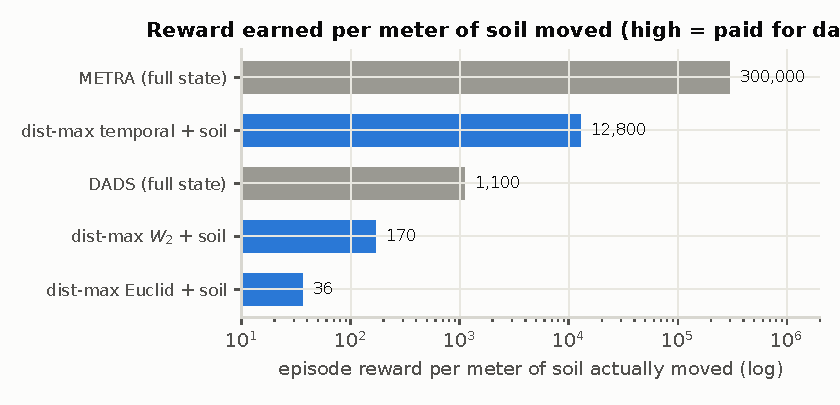
\includegraphics[width=0.74\linewidth]{fig_reward_per_meter.pdf}
\end{center}
{\small The $W_2$ constraint's one surviving virtue: reward in \textbf{physical units} --- the value function is denominated in meters of mass transport. Full-state models earn $\sim$2000$\times$ more reward per unit of real work: paid for dancing.}
\end{frame}

% ============================================================
\section{Demonstration}
% ============================================================

\begin{frame}{The demonstration (live, 3 acts, $\sim$2.5 min, one script)}
\begin{enumerate}
  \item \textbf{``Nobody taught it to dig.''} Four discovered skills cycle on random terrain: dig-and-pile-right, carve-left, excavate-middle, wide-cut. Zero rewards, zero demonstrations, captioned live.
  \item \textbf{``Without our ingredient.''} Split screen, same terrain, same training: soil-only $\phi$ \emph{digs}; full-state $\phi$ (= vanilla METRA) performs elaborate arm choreography over \textbf{untouched soil}. The $8\times$ result, visible in one frame.
  \item \textbf{``Give it a job.''} A red target line appears: \emph{dig the right zone, dump left}. Zero-shot skill steering executes:
  \begin{center}
  \small \ok{\textbf{79\% of the ordered zone's soil removed}}; dump zone filled to within 2.6 points of target; $W_2$ to goal halved --- live counter, before/after cards.
  \end{center}
\end{enumerate}
\medskip
Also available interactively: sculpt terrain with the mouse, record a goal state, wreck it, press ENTER --- with the honest caveat that free-form restoration sits at the method's granularity limit (Exp.\ 8), which we state on-screen rather than hide.
\end{frame}

\begin{frame}{Zero-shot shaping, in full (sim frames $+$ profiles $+$ contraction)}
\begin{center}
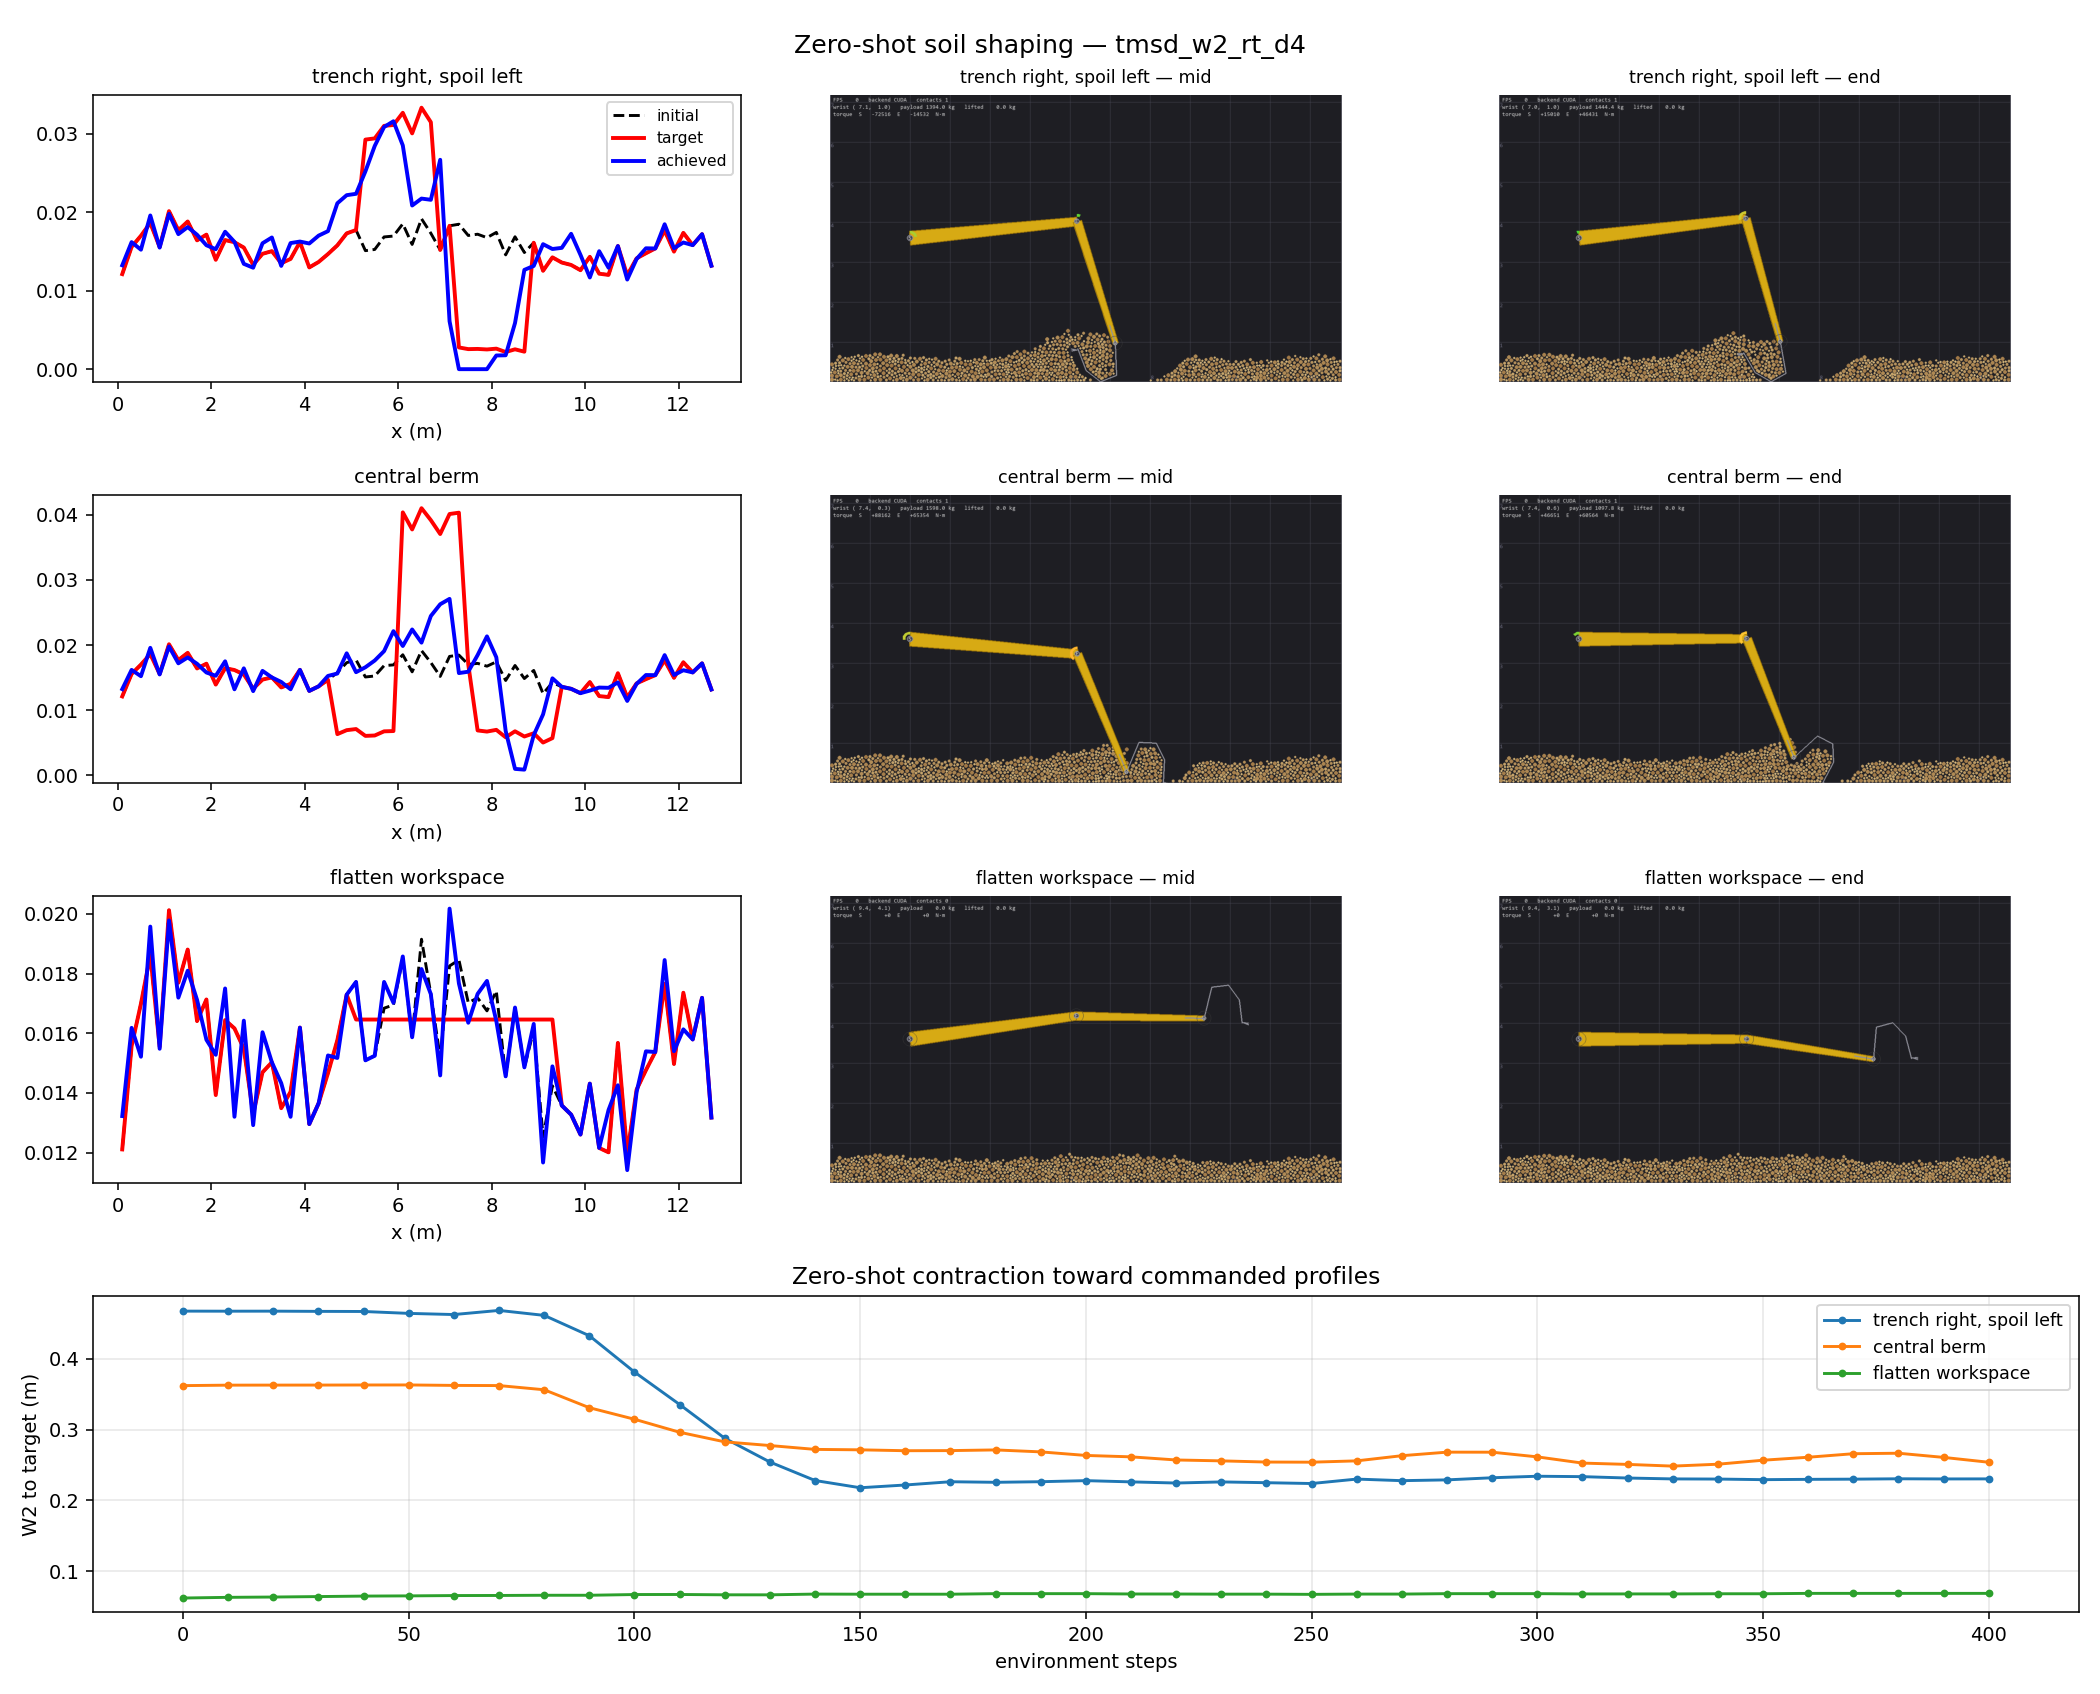
\includegraphics[height=0.82\textheight]{fig_demo_shaping.png}
\end{center}
\end{frame}

% ============================================================
\section{Where this goes}
% ============================================================

\begin{frame}{Contributions (what we can claim today)}
\begin{enumerate}
  \item \textbf{First reward-free skill discovery on granular media} --- digging/piling/shaping emerge with zero supervision (gap confirmed against literature).
  \item \textbf{The two-ingredient law}, with an $8\times$/complete-failure contrast across a $3\times2$ grid, 2--3 seeds per cell: \emph{cumulative} objectives $+$ \emph{external-only} conditioning; each necessary, neither sufficient.
  \item \textbf{Metric-agnosticism} (+ its explanation): on low-dimensional material manifolds, all Lipschitz ground metrics yield the same skills; latent geometry is emergent ($0.99$ isometry to physical $W_2$, unasked). A measured counterpoint to the METRA-lineage emphasis --- and to our own initial bet.
  \item \textbf{Certified zero-shot shaping}: 39--63\% goal-distance reduction, $\sim$90\% monotone contraction, plateau $=$ predicted $r(\varepsilon)$.
  \item \textbf{Slow-state failure taxonomy}: saturation (MI) / starvation (dynamics) / telescoping (distance-max) --- a design law for material-manipulation objectives.
\end{enumerate}
\end{frame}

\begin{frame}{Limits (stated plainly) and next steps}
\textbf{Limits.}
\begin{itemize}
  \item Skill granularity $r(\varepsilon)\approx0.2$\,m: coarse shaping yes, precision restoration no. Diversity $\neq$ controllability.
  \item Fixed machine base $\Rightarrow$ soil transports only \emph{toward} the excavator (like a real backhoe that cannot drive).
  \item One domain family, one simulator, 1D-dominant measure; sliced-$W_2$ starvation unexplained.
\end{itemize}
\textbf{Next.}
\begin{itemize}
  \item \textbf{Second material (dough/plasticine)} --- the generality gate: same objective, unchanged.
  \item \textbf{Mobile base $+$ warm-started goal-conditioned layer} --- closes the reachability and precision gaps for deployment-grade demos.
  \item \textbf{Contraction theorem} --- formalize: $\varepsilon$-coverage of transport directions $\Rightarrow$ geometric $W_2$ contraction to radius $r(\varepsilon)$; the 90\%-monotone data is its empirical half.
  \item Paper: CoRL/RSS empirical spine; theory companion if the certificate formalizes cleanly.
\end{itemize}
\end{frame}

\begin{frame}[standout]
  An excavator taught itself to dig.\\
  We measured \emph{why} that worked ---\\ and why nothing else did.
  \vspace{4mm}

  {\small Demo: \texttt{python scripts/showcase.py}}
\end{frame}

\end{document}
